\subsection{Motor-/sensorstyring}
\subsubsection{Akserne}
Figur \ref{Bipolar} viser test opstillingen af bipolær motor på x-/y-akse, som validerede det forventede resultat, hvor aksen blev flyttet vha. det forøgede moment fra motoren. \\

\begin{figure}[H]
	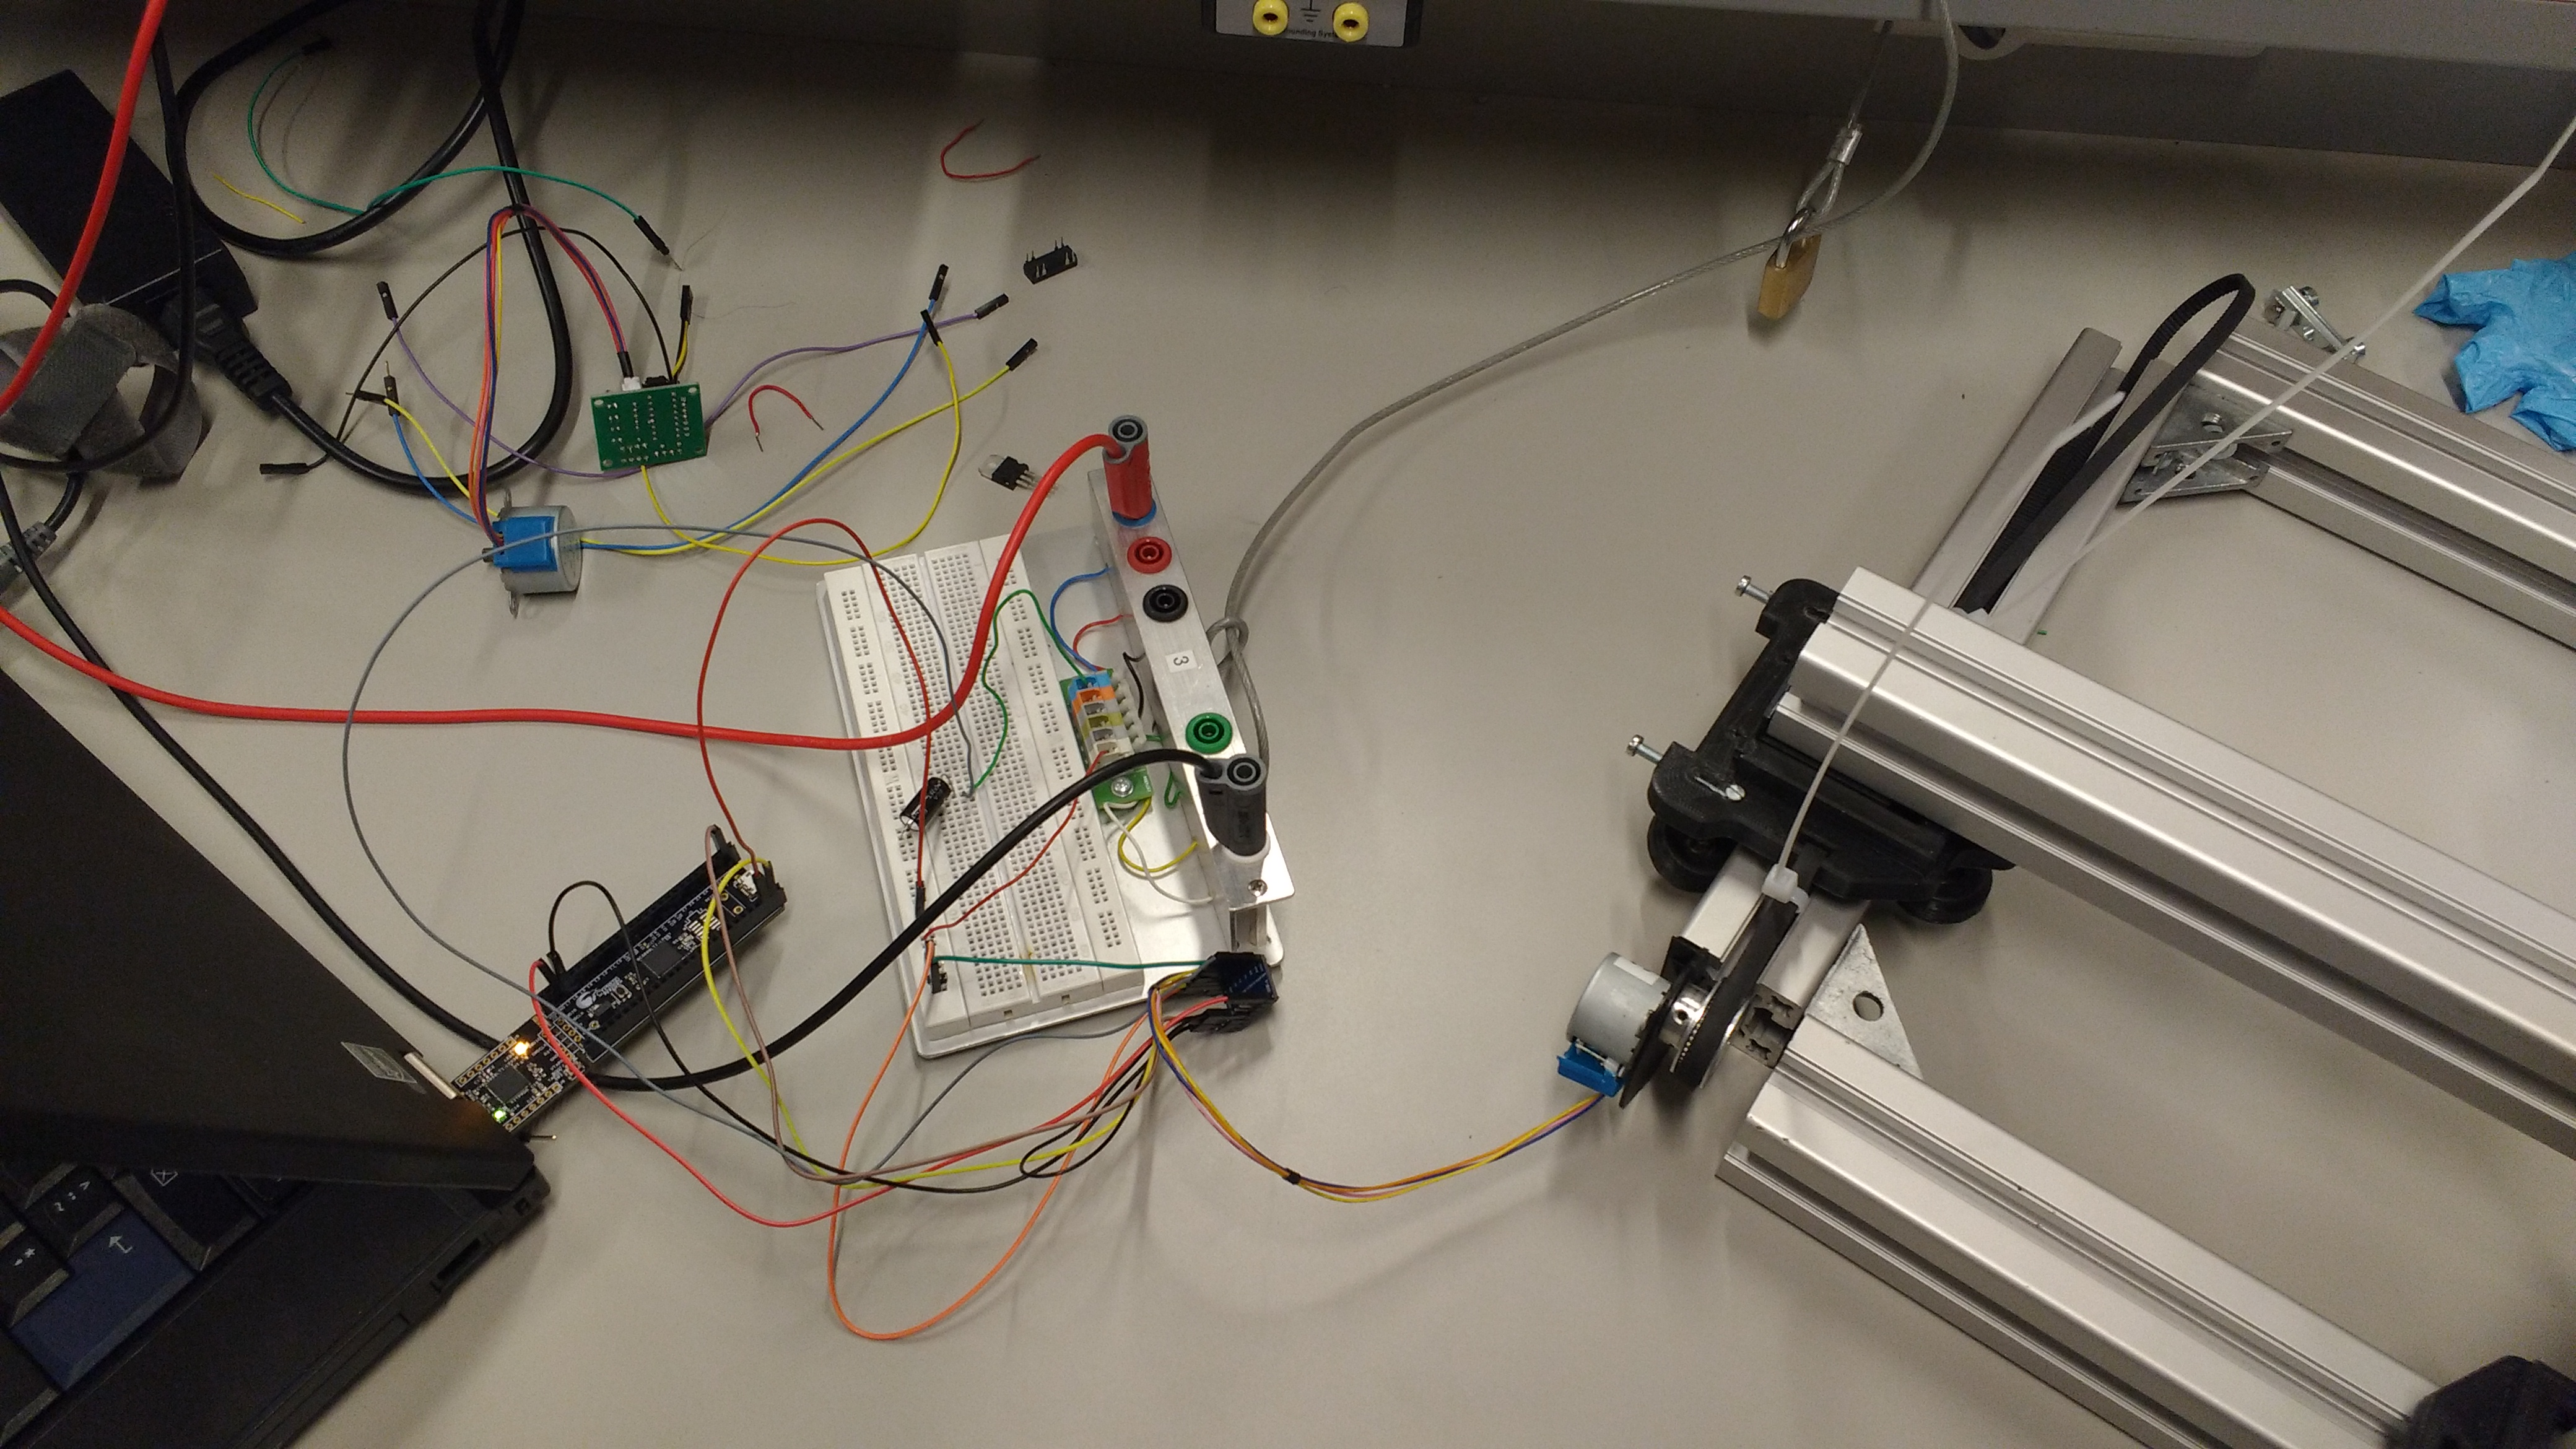
\includegraphics[scale=0.09]{tex/Test/Motor-sensor/Bipolar_test_opstilling.jpg}
	\caption{Test af bipolær motor på x-/y-akse}
	\label{Bipolar}
\end{figure}

Resultaterne fra testen, og andre lignende test af z-aksen (se evt. bilag xx), betød at en udvidet modultest kunne udføres hvori akserne samt detektering foregik. Desværre lykkedes det aldrig at få glidende bevægelser på akserne, som med stor sandsynlighed skyldes konstruktionens ujævnheder. \\

Sensorerne blev testet ved at lade forskellige materialer blive detekteret på afstand af varierende størrelser, hvor det viste sig at sensorerne var ret pålidelige når resultaterne blev holdt op mod Figur 4 i databladet (reference) for dem. Et resultat, målt i mV, kan ses på Figur \ref{Sensor_10cm} under fanebladet Value, ellers henvises til bilag xx for flere resultater. \\

\begin{figure}[H]
	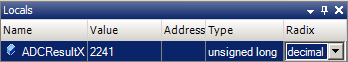
\includegraphics[scale=1]{tex/Test/Motor-sensor/Sensor_10cm.png}
	\caption{Resultat af detektering fra sensor ved 10 cm}
	\label{Sensor_10cm}
\end{figure}

Værdien for detektering ved 10 cm var 2241 mV som lægger sig tæt op ad de ca. 2300 mV der kan udledes af databladet, altså en afvigelse på 2,57\%, eller en unøjagtighed på 2,57 mm ved denne afstand. Sensorernes unøjagtighed ville altså være for stor ift. at en åbningsmekanisme skulle lægge sig over flasken og åbne den.